\section{Zielsetzung}
    Das Ziel dieses Versuchs ist es die Rubidium-Isotope $\ce{^{85}Rb}$ und $\ce{^{87}Rb}$ mittels Hochfrequenzspektroskopie zu untersuchen.\\
    Dafür werden Elektronen durch optisches Pumpen in angeregte Zustände versetzt. Diese Zustände lassen sich dann mittels radio-frequenten magnetischen Feldern untersuchen.
\section{Theorie}

\subsection{Energielevelstruktur des Rubidium-Atoms}

\noindent
Das Rubidium-Atom gehört zu ersten Hauptgruppe. Das Heißt, dass es nur ein Elektron in der äußersten Schale besitzt.\\
Dies macht es sehr geeignet für diesen Versuch, da damit nur ein Elektronenspin beachtet werden muss.\\
Der Unterschied zwischen den beiden Isotopen sind ihre Kernspins $I$. 
$\ce{^{85}Rb}$ hat einen Kernspin von $I = \frac{5}{2}$ und $\ce{^{87}Rb}$ von $I = \frac{3}{2}$.\\ 
Der Aufbau inklusive Spins ist auch in Abbildung \ref{img:Iso} noch einmal dargestellt.

\begin{figure}[H]
    \centering
    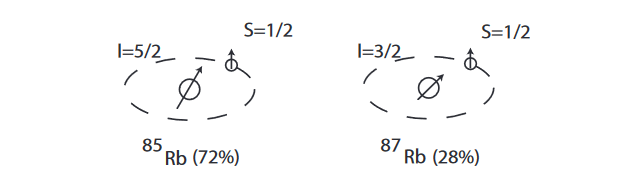
\includegraphics[width=0.6\textwidth]{latex/images/Isotopes.PNG}
    \caption{Die Rubidium-Isotope und ihre Spins schematisch dargestellt\protect \cite{pump_1}.}
    \label{img:Iso}
\end{figure}

\noindent

